\documentclass[12pt]{article}
\usepackage[spanish]{babel}
\usepackage[utf8]{inputenc}
\usepackage{graphicx}
\usepackage{amsmath}
\usepackage{booktabs}
\usepackage{float}
\usepackage{hyperref}
\usepackage[a4paper, margin=2.5cm]{geometry}
\usepackage{setspace}
\setstretch{1.15}

\title{Taller 3b – Análisis de Componentes Principales (PCA)}
\author{Estudiante: Juan Felipe Gómez Carmona \\ 
Maestría en Analítica Aplicada \\
Universidad de La Sabana \\ 
Profesor: Hugo Franco, Ph.D.}
\date{Octubre 2025}

\begin{document}

\maketitle
\tableofcontents
\newpage

\section{Introducción}
Este taller tiene como propósito aplicar la técnica de \textbf{Análisis de Componentes Principales (PCA)} dentro de un flujo de trabajo de aprendizaje supervisado. A través de los datasets \textit{Iris} y \textit{Wine Quality}, se busca analizar el efecto de la reducción de dimensionalidad sobre el rendimiento de modelos \textit{k-NN}, tanto en problemas multiclase como binarios. 

El objetivo central es comprender cómo el PCA transforma los datos originales en nuevas variables (componentes principales) que concentran la mayor cantidad de varianza posible, reduciendo la complejidad sin sacrificar significativamente la capacidad predictiva. 

\section{Metodología}

\subsection{Dataset y Preprocesamiento}
\textbf{Iris Dataset:} contiene 150 muestras de tres especies de flores (\textit{Setosa, Versicolor, Virginica}) con cuatro características morfológicas. Se utiliza para demostrar la reducción de dimensionalidad y la visualización 2D mediante PCA.

\textbf{Wine Quality Dataset:} incluye 1599 muestras de vino tinto, con 11 variables fisicoquímicas y una etiqueta de calidad numérica. Esta variable se transformó en tres categorías: \textit{Poor, Fair y Good}, y posteriormente en una clasificación binaria (\textit{Good} > 6).

Los datos fueron divididos en entrenamiento (80\%) y prueba (20\%), aplicando escalamiento con \texttt{StandardScaler} antes del PCA.

\subsection{Procedimiento}
El flujo de trabajo seguido fue:
\begin{enumerate}
    \item Entrenar un modelo base (\textit{k-NN}) sin PCA.
    \item Aplicar PCA y repetir el entrenamiento con 2 componentes.
    \item Evaluar el desempeño mediante \textit{accuracy, recall, precision}.
    \item Visualizar la varianza explicada y las proyecciones 2D.
    \item Extender el análisis al caso binario (\textit{Good > 6}).
\end{enumerate}

\section{Resultados}

\subsection{Iris Dataset}
\begin{figure}[H]
\centering
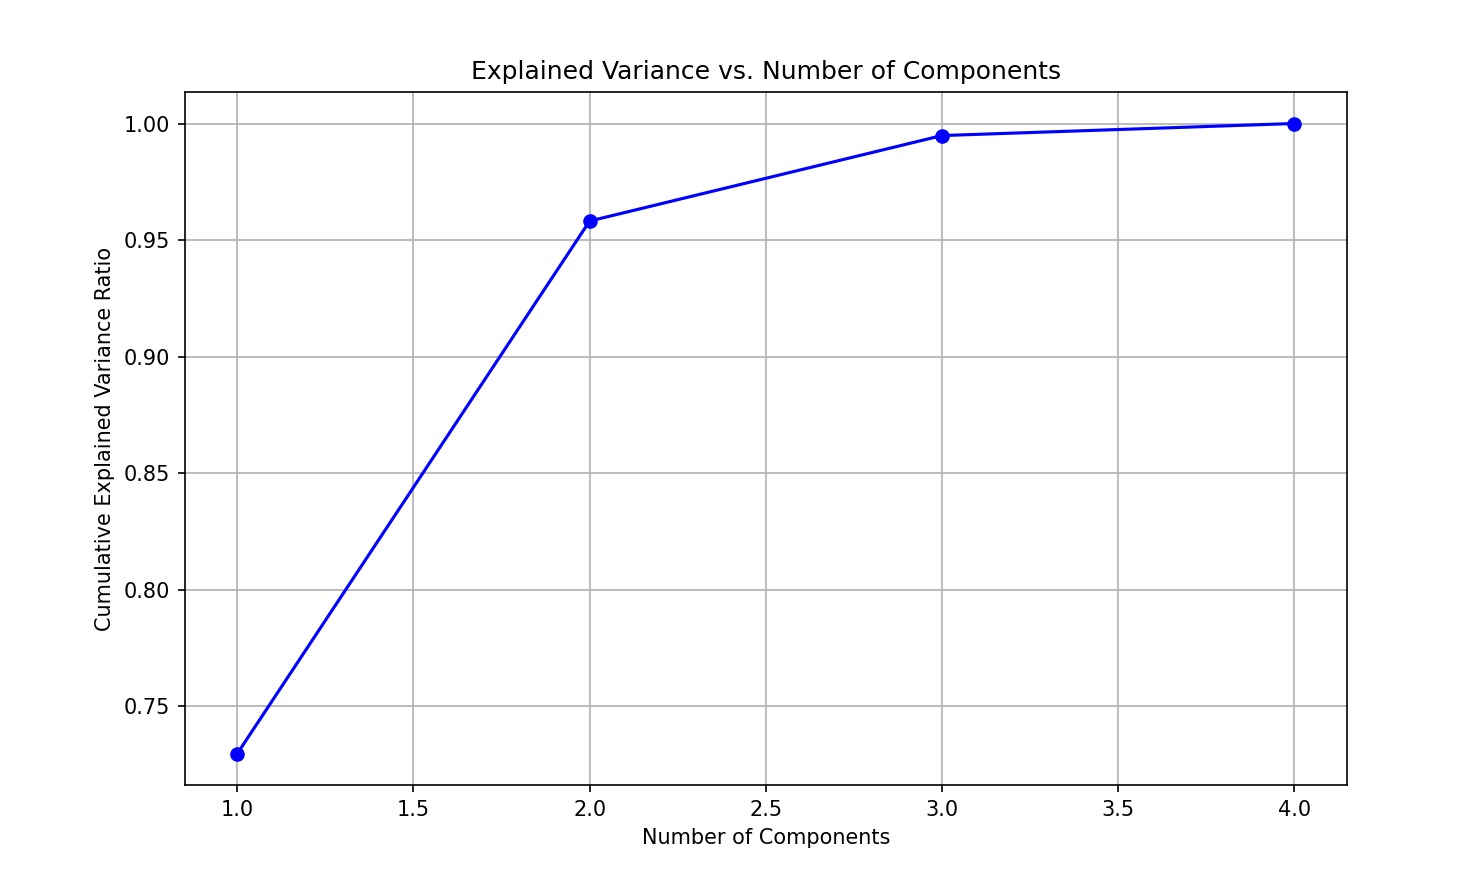
\includegraphics[width=0.7\textwidth]{figures/iris_explained_variance.png}
\caption{Varianza explicada acumulada según el número de componentes (Iris Dataset).}
\end{figure}

\begin{figure}[H]
\centering
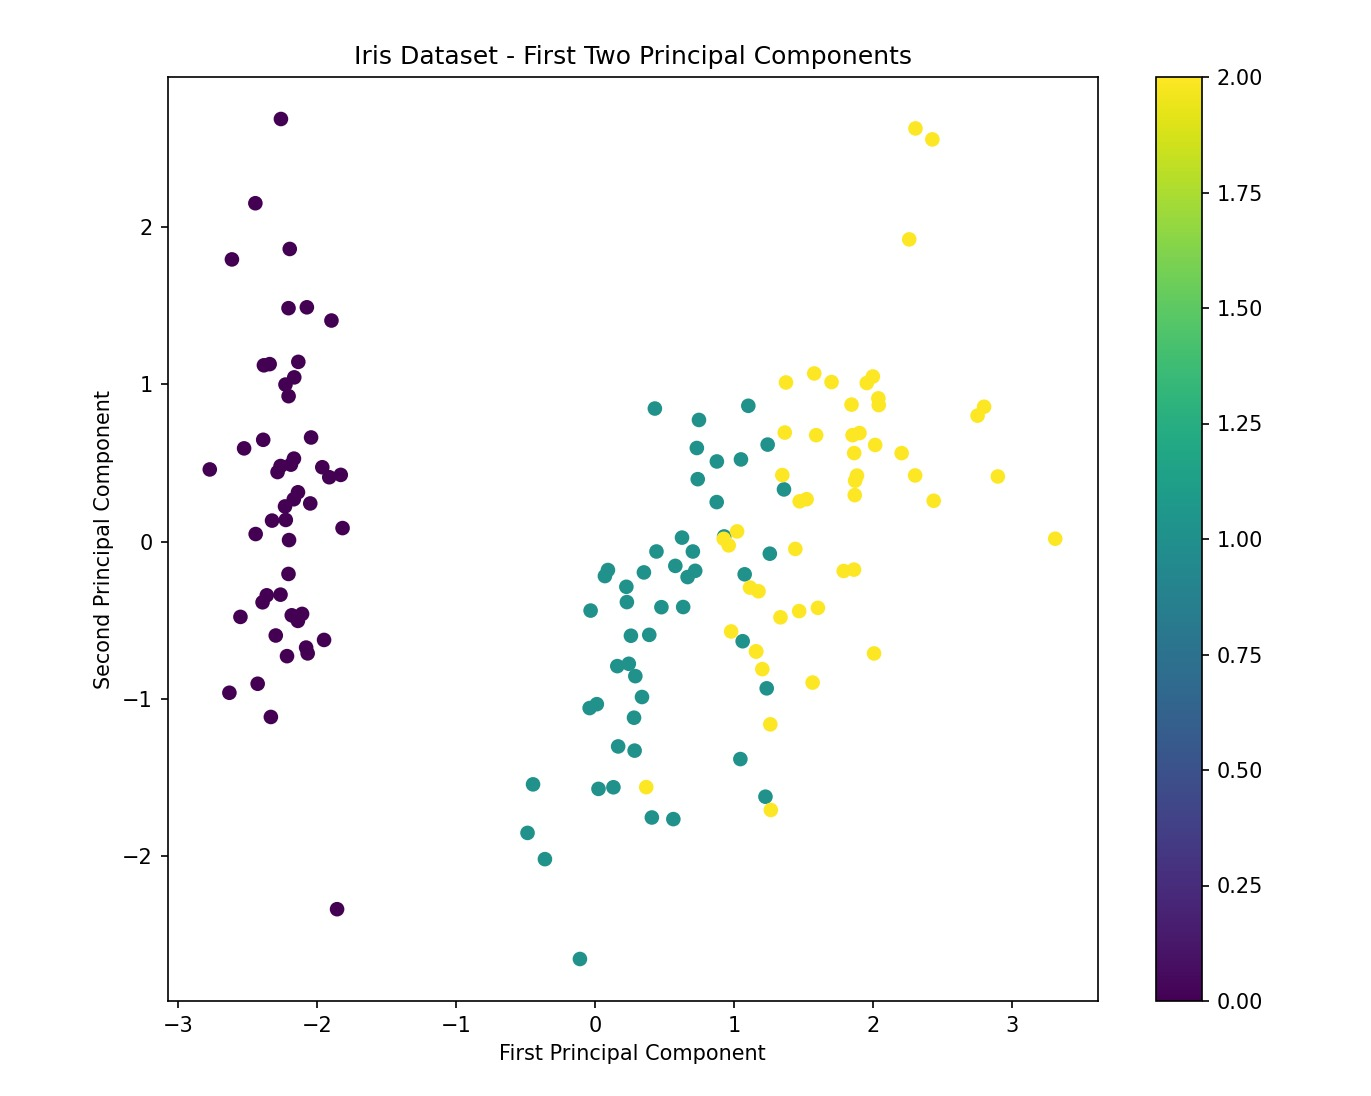
\includegraphics[width=0.7\textwidth]{figures/iris_pca_projection.png}
\caption{Proyección 2D del Iris Dataset en los dos primeros componentes principales.}
\end{figure}

El modelo PCA alcanzó una precisión similar al modelo base, mostrando que la información principal del Iris se retiene en las dos primeras dimensiones (\textasciitilde95\% de la varianza). Esto evidencia que PCA es altamente eficiente cuando las variables originales están fuertemente correlacionadas, como ocurre en este conjunto.

\subsection{Distribución y Varianza – Wine Dataset}
\begin{figure}[H]
\centering
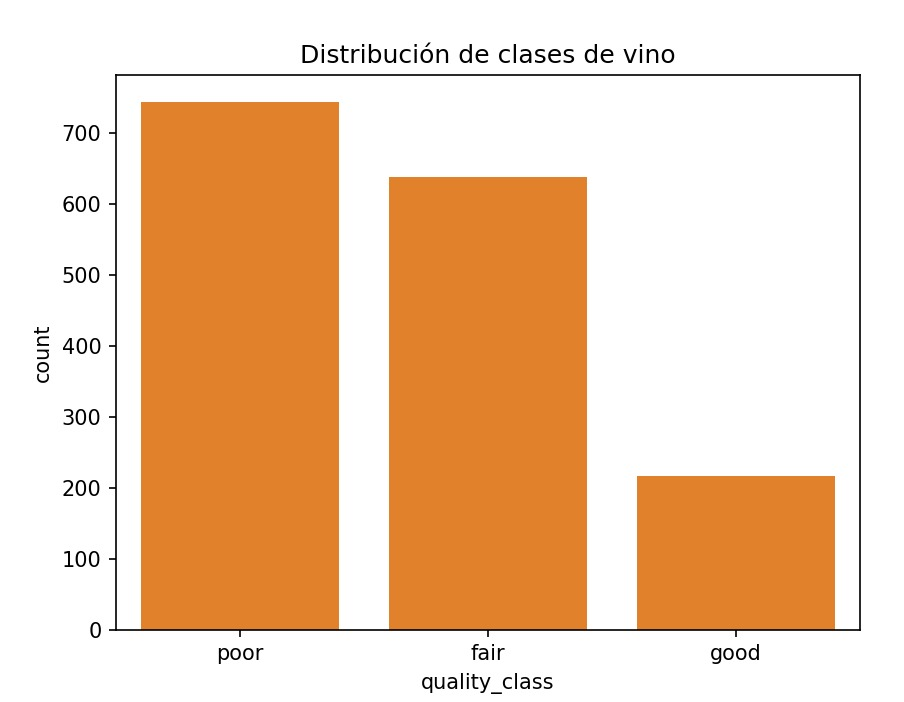
\includegraphics[width=0.7\textwidth]{figures/wine_class_distribution.png}
\caption{Distribución de clases en el dataset de vino tinto.}
\end{figure}

\begin{figure}[H]
\centering
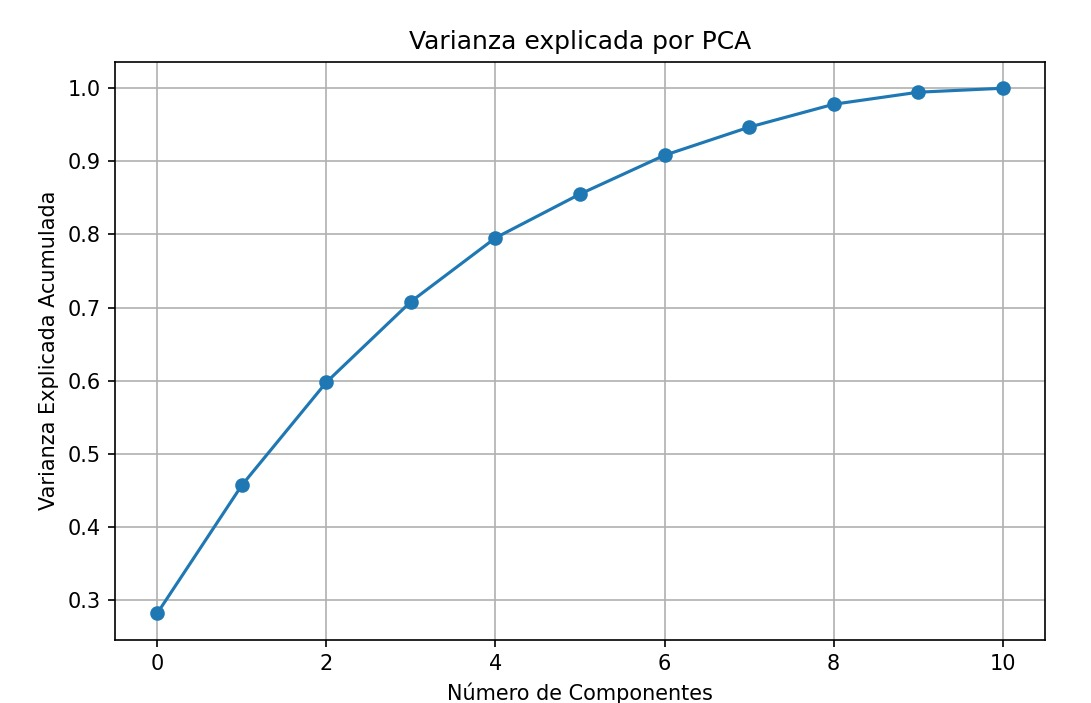
\includegraphics[width=0.7\textwidth]{figures/wine_explained_variance.png}
\caption{Varianza explicada acumulada por número de componentes (Wine Dataset).}
\end{figure}

Las dos primeras componentes retienen aproximadamente el 46\% de la varianza total, lo que implica una pérdida de información relevante para la clasificación. A diferencia del Iris, este conjunto presenta alta multicolinealidad y mayor complejidad, por lo que PCA no logra capturar de manera compacta toda la estructura informativa.

\subsection{Visualización PCA 2D – Wine Dataset}
\begin{figure}[H]
\centering
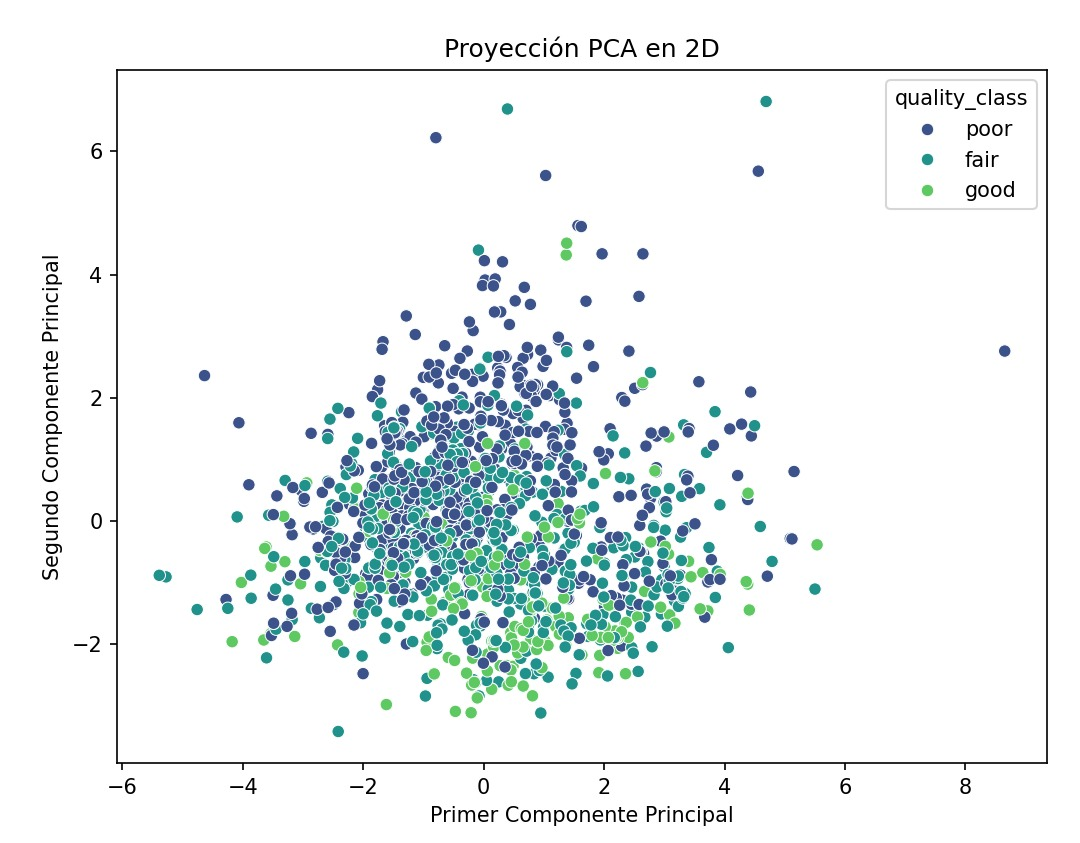
\includegraphics[width=0.7\textwidth]{figures/wine_pca_projection.png}
\caption{Proyección PCA en 2D del Wine Dataset.}
\end{figure}

Las clases \textit{poor}, \textit{fair} y \textit{good} presentan una alta superposición, reflejando la dificultad del modelo para separar clases de calidad similares en un espacio reducido de dos dimensiones. Esto refuerza la idea de que PCA, aunque útil para exploración visual, no siempre mejora el poder discriminativo.

\subsection{Desempeño de Modelos}
\begin{table}[H]
\centering
\begin{tabular}{l c c}
\toprule
\textbf{Modelo} & \textbf{Exactitud (Accuracy)} & \textbf{Tipo de Clasificación} \\
\midrule
Base (sin PCA) & 0.55 & Multiclase \\
Con PCA (2 comps.) & 0.52 & Multiclase \\
Base Binario & 0.86 & Binaria \\
PCA Binario (2 comps.) & 0.86 & Binaria \\
\bottomrule
\end{tabular}
\caption{Comparación general de desempeño entre modelos con y sin PCA.}
\end{table}

En la clasificación binaria, los modelos mejoran considerablemente su exactitud (86\%), confirmando que la simplificación del problema reduce el error de clasificación.

\section{Discusión}
Los resultados evidencian que el PCA:
\begin{itemize}
    \item Facilita la \textbf{visualización} y simplifica el modelo, aunque con pérdida de información relevante en datasets complejos.
    \item No mejora el rendimiento predictivo en el problema multiclase, ya que las relaciones no lineales entre variables no se capturan adecuadamente en componentes lineales.
    \item En la versión binaria, conserva una precisión alta, manteniendo eficiencia computacional sin comprometer el rendimiento.
\end{itemize}

Además, al comparar los resultados entre los dos conjuntos de datos, se pueden notar diferencias claras:

\begin{itemize}
    \item En el caso del \textbf{Iris Dataset}, los datos están bien organizados y las clases se distinguen con facilidad. Esto hace que el PCA funcione muy bien, ya que con solo dos componentes logra conservar casi toda la información importante del conjunto.
    \item En cambio, el \textbf{Wine Quality Dataset} es mucho más complejo. Las clases no están tan separadas y las variables se relacionan de forma más enredada. Al reducir los datos a solo dos componentes, se pierde parte de la información necesaria para distinguir bien los vinos de diferente calidad.
    \item Esto muestra que el PCA no siempre es la mejor opción. Su utilidad depende mucho del tipo de datos que se esté analizando y del objetivo del trabajo: si se busca entender mejor los datos y visualizarlos, el PCA ayuda bastante; pero si lo que se necesita es la máxima precisión posible, puede no ser suficiente por sí solo.
\end{itemize}

\section{Conclusiones}
\begin{itemize}
    \item El PCA es útil para exploración y reducción de dimensionalidad, aunque no siempre mejora la exactitud de los modelos predictivos.
    \item En el caso multiclase, la pérdida de información fue significativa (solo 46\% de varianza retenida), afectando la capacidad del modelo.
    \item La clasificación binaria mejora notablemente la precisión general (86\%), evidenciando la importancia de simplificar el problema cuando es posible.
    \item Se recomienda usar PCA como herramienta de apoyo para visualización, análisis de correlaciones y eficiencia, más que como optimizador de modelos.
\end{itemize}

\section{Referencias}
\begin{itemize}
    \item UCI Machine Learning Repository. (2025). \textit{Wine Quality Dataset}. Disponible en: \url{https://archive.ics.uci.edu/ml/machine-learning-databases/wine-quality/}
    \item Scikit-learn Documentation. (2025). \textit{Decomposition: PCA}. Disponible en: \url{https://scikit-learn.org/stable/modules/generated/sklearn.decomposition.PCA.html}
\end{itemize}

\end{document}
